\documentclass{article} % For LaTeX2e
\newcommand{\argmin}{\arg\!\min}
\usepackage{mathtools}
\usepackage{amsmath}

\usepackage{graphicx}
\usepackage{epstopdf} %%package to overcome problem with eps in pdf files
\usepackage{array} 
\usepackage{booktabs}
\usepackage{multirow}
\usepackage{siunitx}
\usepackage{colortbl}
\definecolor{kugray5}{RGB}{224,224,224}
\usepackage{graphics}
\usepackage{caption}
\usepackage{subcaption}
\usepackage{geometry}

\DeclarePairedDelimiter\ceil{\lceil}{\rceil}

\usepackage{nips14submit_e,times}
\usepackage{hyperref}
\usepackage{url}
%\usepackage[top=5mm]{geometry}
\usepackage[ bibstyle=numeric,, maxnames=1, backend=bibtex]{biblatex}
\addbibresource{ml_project.bib}
%\documentstyle[nips14submit_09,times,art10]{article} % For LaTeX 2.09


\title{A Supervised Learning Based Approach for block page Detection}

\author{
Arian Akhavan Niaki\\
College of Information and Computer Sciences\\
University of Massachusetts\\
140 Governors Dr., Amherst, MA 01003 \\
\texttt{arian@cs.umass.edu} \\
}
% The \author macro works with any number of authors. There are two commands
% used to separate the names and addresses of multiple authors: \And and \AND.
%
% Using \And between authors leaves it to \LaTeX{} to determine where to break
% the lines. Using \AND forces a linebreak at that point. So, if \LaTeX{}
% puts 3 of 4 authors names on the first line, and the last on the second
% line, try using \AND instead of \And before the third author name.

%\newcommand{\fix}{\marginpar{FIX}}
%\newcommand{\new}{\marginpar{NEW}}

%\nipsfinalcopy % Uncomment for camera-ready version

\begin{document}
\maketitle

\begin{abstract}
Current supervised learning approaches in machine learning literature have mostly concentrated on a single aspect data such as images or text, in which they use this data to train their neural network. However, combining these two data could improve performance in the case of missing data in either images or text. In this paper, we design and implement a deep convolutional neural network (CNN) which takes both the images and text data in order to do block page detection. We compare our results to an image classification CNN, a text classification CNN and previous heuristic based block page detection. We show that our model achieves a macro-averaged F1 score of 0.981 which is better than the text's 0.985 but slightly worse than the image CNN's score of 0.985.
\end{abstract}
\section{Introduction}
Extensive work has been done in supervised and unsupervised learning on both image and text classification. However, to the best of our knowledge, there does not exist an approach that applies supervised learning on a dataset containing both images and textual data. This can be advantageous in the case where we either have missing data in the images or text. We see this case occurring in the field of Internet censorship and Tor discrimination where various crawlers fail to fetch both the screenshot and the HTML document of the web page.\\
Internet censorship often manifests in the form of \emph{blocked web pages} returned to users accessing content. These blocked pages vary in appearance and content depending on the country. 
Moreover, previous work has shown that users using anonymity systems such as Tor to access the Internet, receive discrimination in multiple forms such as CAPTCHAs, interaction based discrimination, and block pages. \\
Researchers have made attempts to characterize Internet censorship by detecting block pages automatically. However, their efforts have largely been heuristic based and have shortcomings in distinguishing server errors from block pages.\\
In this paper, In order to detect and classify block pages and accurately measure discrimination against users, we use a Selenium-based crawler to fetch the Alexa top 500 websites from 50 Tor exit relays. We then design and implement a deep neural network which leverages both images and the HTML text of the web pages in order to do multi-class classification by detecting block pages, server errors, connection errors, and legitimate web pages. In order to measure the performance and accuracy of our proposed model, we perform three experiments comparing the precision, recall, F1 score and macro-averaged F1 score of our model to a case where we use a state-of-the-art image classification deep neural net, a text classification deep neural net separately and heuristic based block page detection. We show that our proposed model can achieve better performance compared to the text CNN but is slightly outperformed by the image CNN. 
\section{Related Work}
As there is no related work on block page detection using machine learning techniques, in this section, we describe related work in image and text classification and prior work done in block page detection using heuristic techniques.

\subsection{Image Classification}
One of the most cited works done in image classification is ImageNet~\cite{imagehinton}. The structure of our image classification deep neural network is inspired by this work. However, our proposed network also receives a text document as input while this work only concentrates on images.
The authors trained a large, deep convolutional neural network to classify 1.2 million high-resolution images into 10 different classes. In contrast, our network is designed to classify into 4 different classes.
They implement their model using parallel GPUs and show that the best number of layers for their task is five convolutional layers followed by max-pooling layers and three fully-connected layers. Some of the other advances they proposed was using Rectified Linear Units (ReLUs) as the linear activation unit in their neural network which makes training six times faster than the alternative $f(x) = tanh(x)$.Their model's architecture is shown in Figure~\ref{fig:imagenet}.
\begin{figure}
\centering
        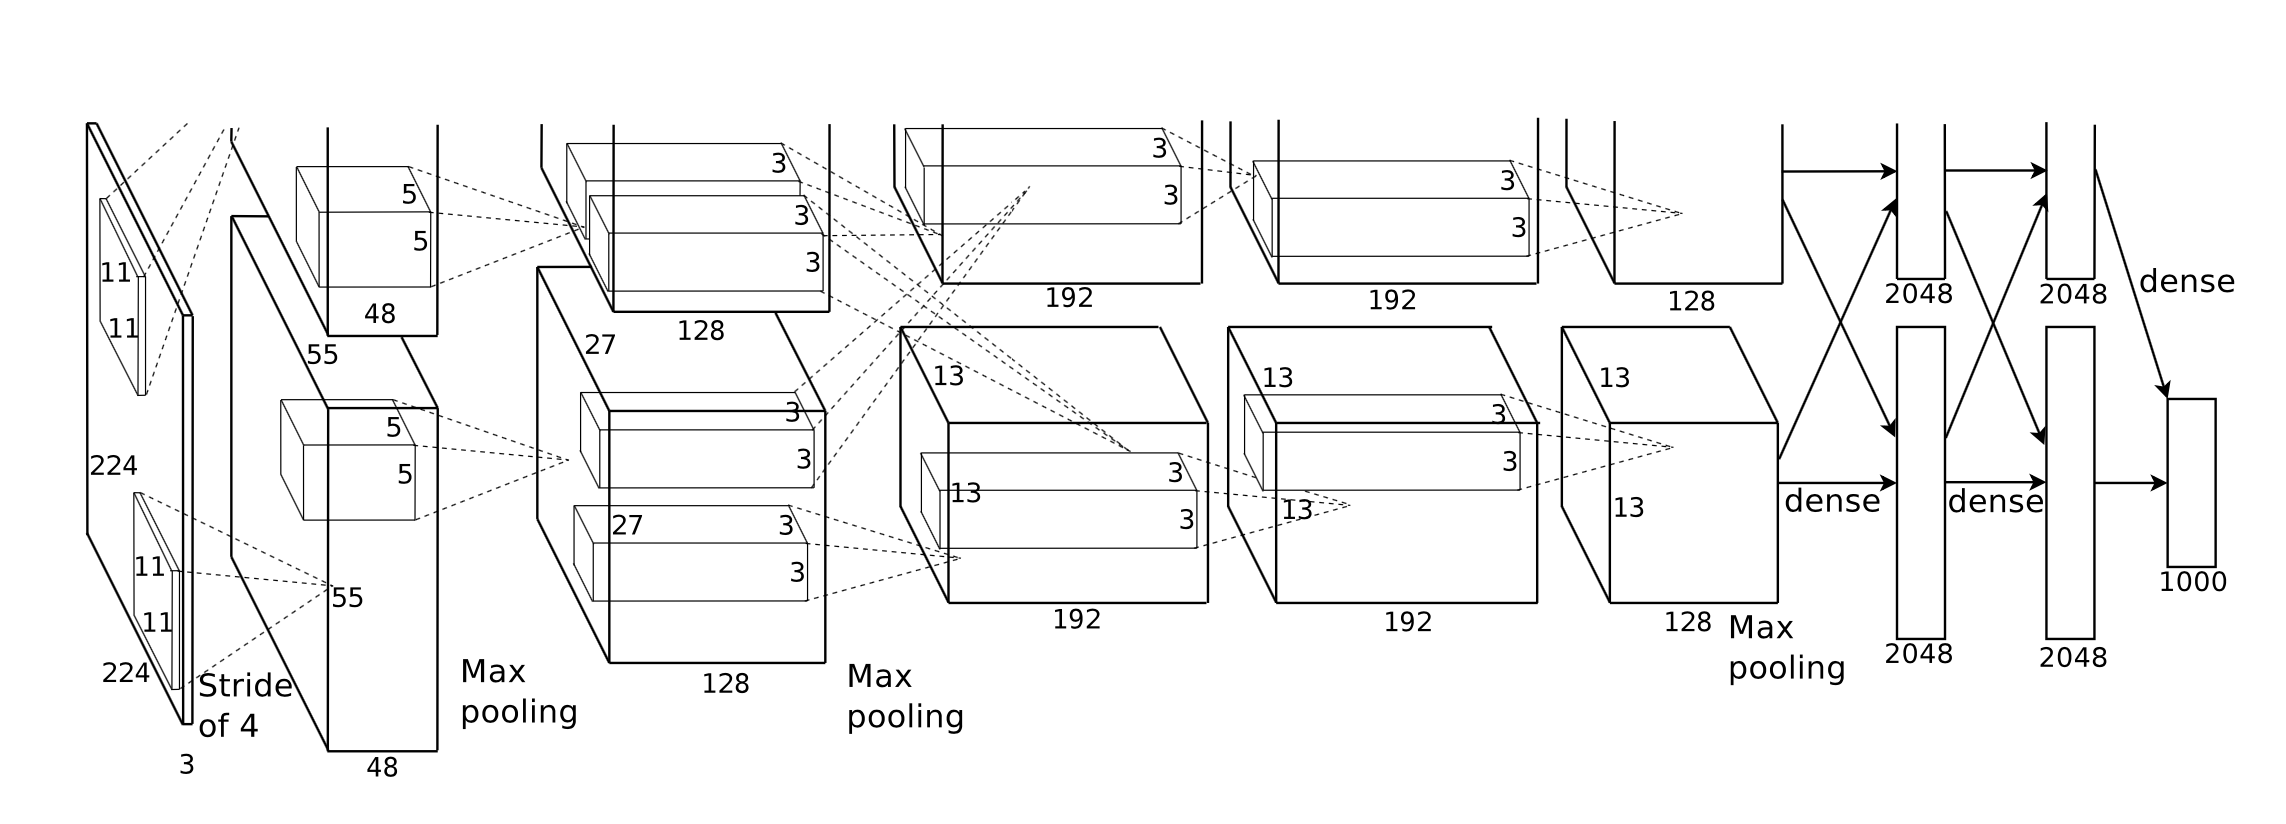
\includegraphics[totalheight=5cm]{imagenet}
    \caption{Imagenet architecture \protect\cite{imagehinton}}
    \label{fig:imagenet}
\end{figure}
They solve overfitting using (1) data augmentation which artificially enlarges the dataset using transformations on images and (2) applying dropout where they set the output of each hidden neuron to zero with 0.5 probability. These dropped neurons do not contribute to the forward pass and the backpropagation and the model learns more robust features.
One weakness of this paper is not declaring the decision behind the parameters of the neural network architecture. They also do not provide numerical results for the effects of different dropout probabilities. However, this deep neural network would not work with our dataset. Our work complements this by adding a neural network for text classification as well and we suspect it will perform better in the case where image data is missing but we have the HTML of the web page.

The authors of ~\cite{nipsandrewng} have introduced an extension to convolutional neural networks (CNN) called Tiled CNNs. Rather than all weights being equal, these networks only require hidden units positioned k steps of each other to have equal weights which will lead to learning more complex range of invariances. 
They also use an unsupervised learning algorithm that learns features from unlabeled image patches called Topographic ICA (TICA). They show that TICA pretraining for Tiled CNNs performs well on object recognition. We explain in section~\ref{sec:discussion}, how this work can be integrated into our proposed network. However, a weakness of this paper is that they experiment on a limited number of datasets.

Authors in ~\cite{icml_unsupervised} show that one can build high-level, class-specific feature detectors from unlabeled in an inexpensive way. This is an extension to autoencoders which are used for learning low-level features. They use a large dataset of 200x200 images and feed it into a deep autoencoder with pooling and local contrast normalization. They employ local receptive fields,  local contrast normalization, and local l2 pooling to scale for larger images and learn invariant features. Although our dataset contains only labeled data, we can use unlabeled data to learn high-level features and then train our network using labeled data. We will discuss how we can integrate this work with ours in section~\ref{sec:discussion}.

\subsection{Text Classification}
\begin{figure}
\centering
        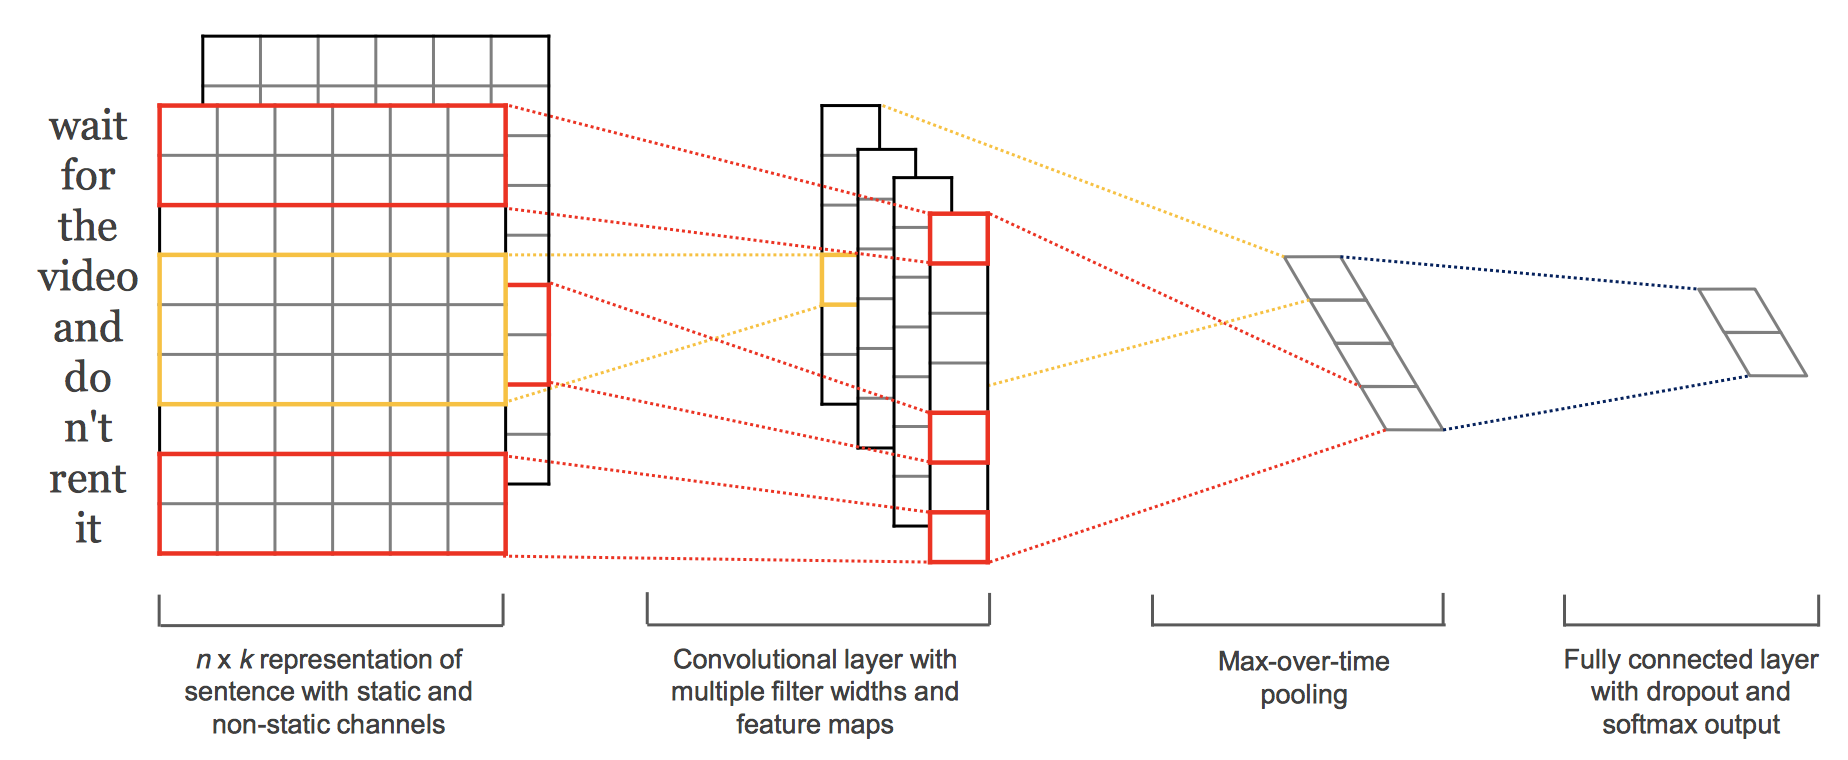
\includegraphics[totalheight=3cm]{textnet}
    \caption{Architecture of text classification CNN \protect\cite{convtext}}
    \label{fig:textnet}
\end{figure}
There exists a myriad of publications on text classification. The goal of text classification is to assign free-text documents to predefined categories. In ~\cite{convtext}, authors demonstrate that applying a CNN on top of a pre-trained word vector performs well on sentence-level classification tasks. They train a CNN with a single layer of convolution on top of word vectors that are pre-trained on 100 billion words of Google News\footnote{https://code.google.com/p/word2vec/}. The results suggest that pre-trained vectors are universal feature extractors. Their model's architecture is shown in Figure~\ref{fig:textnet}. The structure of our proposed text CNN is inspired by this work. They apply regularization by using dropout on the ouput of the max pooling layer. One of their strong points in this work is performing experiments using several variants of the model. For example comparing the result of a CNN with static pre-trained vectors, and CNN with randomly initialized words vectors on multiple datasets. However, this model would not work on our dataset because we have images in addition to HTML documents. Additionally, this model fails to work with pages which have words not available in the embedding matrix. We complement this model by adding a neural network for image classification which will help in the cases where text is missing in our data.
%In their model a sentence of length $n$ is represented as: $x_{1:n} = x_1 \oplus x_2 \oplus ... \oplus x_n$ and $x_i$ is the k-dimensional word vector for the i-th word. They apply a convolutional operation to a window of $h$ words to produce a new feature. $c_i = f(w\cdot x_{i:i+h-1} + b)$ where $f$ is a non-linear function. Therefore a feature map $c = [c_1, c_2, ...,c_{n-h+1}]$ is constructed, after this a max pooling operation is applied over this feature map where it outputs $\hat{c} = max(c)$ capturing the most important features for each feature map. These features are then passed to a fully-connected  layer. The output of the softmax layers is the probability distribution over labels. The model uses multiple filters with different window sizes to obtain multiple features. Regularization is applied by using dropout on the output of the max pooling layer. One of their strong points is performing experiments using several variants of the model. For example comparing the result of CNN with static pre-trained vectors, and CNN with randomly initialized words vectors on multiple datasets. This deep neural network would not also work with our dataset because it contains text in addition to images. Our work complements this by adding a neural network for image classification as well and will presumably perform better in the case where text data is missing but we have the image of the web page.
%

Character-level CNNs for text classification is studied in ~\cite{nips_text}. They consider text as a raw signal at the character level and apply one-dimensional CNNs to it. An alphabet of size $m$ is constructed and each character is encoded to a one-hot vector with a fixed length $l_0$. Characters not present in the alphabet are set to all-zero vectors. One strong aspect of this paper is applying data augmentation using a thesaurus and replacing words by their synonyms to control generalization error. They compare their results to word-based CNN approach described in ~\cite{convtext} as well as traditional text classification models such as bag-of-means on word embeddings. They conclude that the model performance depends on various factors such as dataset size and choice of the alphabet and show that character-level CNN could work for text classification without needing words.

Finally, a work done by ~\cite{nn_survery} performs a survey on neural network models from the perspective of natural language processing research. Specifically related to our work is their discussion on convolutional neural networks and the use of word embeddings for representing each feature as a vector in a low dimensional space. According to ~\cite{nn_survery} convolutional networks with pooling layers perform well in classification tasks. The strong point of this work that it does a comprehensive study on different aspects of neural network models for natural language processing. However, it does not provide sufficient details about each approach. We have designed our text classification neural network while having in mind that CNNs are to be integrated into larger networks in order to be effective ~\cite{goldberg2017neural}.
\subsection{Block page detection}
~\parencite{imc14_phillipa} propose length differences between a censored page and its uncensored counterpart as a heuristic, 
relying on the idea that blocked pages usually shorter than the original page. However, this approach fails to distinguish server errors from block pages and connection errors. Whereas, our model is designed to distinguish them accurately.
We did not find research on blocked page detection in the field of machine learning, however, machine learning techniques have been used for detecting website defacements by ~\parencite{meerkat}. The structure of their deep neural network was inspired by work from~\parencite{imagehinton}, \parencite{nipsandrewng}, and ~\parencite{icml_unsupervised}.

\section{Methodology}
In this section, we describe the architecture of our convolutional neural network for classifying web pages into 4 classes. Our model consists of the two previously mentioned parts that run in parallel. The novelty of our approach is that we consider both data cases of image and text at the same time. This will prove advantageous when we have missing data, either not having the HTML document or not having the screenshot. This happens in our data set as well, we have data cases where an error occurred and the HTML document is blank but we have a screenshot of the error page. We implement our neural network in Python using the tensorflow library~\cite{tensorflow2015}. Another case where our proposed model will work better than previous text classification models is that if the web page contains words that are not in the pre-trained word vector matrix. In these cases, our model uses the screenshots to make the prediction whereas a simple text classification CNN would fail.

\subsection{Image Neural Network}
The design of our image classification convolutional neural network is inspired by ~\cite{imagehinton} and consists of 5 layers. More specifically, the first three layers are convolutional layers and the final two are fully-connected layers. Since we have 44 categories, the output of the last fully-connected layer is given as input to a $4$-way softmax function shown in ~\ref{softmax} which predicts the class labels. We use the softmax cross-entropy described in \ref{crossentropy} as our cost function.
\begin{equation} \label{crossentropy}
\theta_{*} = \argmin_\theta \sum_{n=1} ^{N} -y \times log(p)-(1-y)\times log(1-p)
\end{equation}

For optimizing the cost function we employ the Adam algorithm. According to empirical results, it achieves better results in comparison to other stochastic optimization methods ~\cite{adam}. Our first convolutional layers filter the $160\times160\times3$ input images with $32$ kernels of size $16\times16\times3$ with a stride of $4$ pixels which means we slide the convolutional filter over the input image by $4$ pixels at a time, this will reduce the size of the CNN's output. Further, we want the output of the CNN to have the same size as the input, therefore we apply zero padding where $0$ values are added to the edge of the input to preserve the input size. We use the ReLU activation function $f(x) = max(0,x)$ for the outputs of the CNN neurons as it is shown to be faster than the alternative $tanh$ activation function~\cite{imagehinton}. We then apply a $2\times2$ max-pooling where we select the largest value from each $2\times2$ window. 
The second and third layers filter the output of their previous layer using $64$ kernels of size $8\times8\times3$ and $128$ kernels of size $4\times4\times3$ with a stride of $4$ pixels, $2\times2$ max pooling, and ReLU activation functions, respectively. As ~\cite{CNNdropout2} has shown that using dropout in convolutional neural networks improves performance, we have also done the same.
Finally, we flatten the output of the third convolutional layer in order to make it suitable as input to the fully-connected layers with $128$ neurons. In order to avoid overfitting, we apply dropout to our fully-connected layers. Prior work has also shown that using dropout on the last hidden layer of a fully-connected layer reduces the error rate ~\cite{CNNdropout}. To be more concise, we set zero the output of each hidden neuron with probability 0.5. By doing this, we make sure that the network is not always using the same neurons and is not getting fitted to the training data. The output of the last fully-connected layer will go through a $4$-way softmax function if we want to run the network separately as we do in section~\ref{experiments}. The network's architecture is shown in the top part of 
~\ref{fig:CNN}. The full network structure is available in the appendix.

\begin{equation}
  \label{softmax}
  P(y=j | x) = \frac{\exp(x^T w_j)}{\sum^{N}_n=1 \exp(x^T w_n))},
\end{equation}

\subsection{Text Neural Network}
The design of our text classification CNN is inspired by~\cite{convtext}. Similar to our image classification neural net, it consists of 5 layers, with the first three being convolutional networks and the rest being fully-connected layers. We need to apply some pre-processing on our HTML data in order to extract features before we can input them to the network. First, we separate the \textit{body} section of the HTML pages then we only consider the first $200$ words of the body $doc=[w_1,w_2,...w_{200}]$. In order to convert these words into features, we use pre-trained word vectors from GloVe's embedding matrix which contains 300-dimensional vectors for $1.9$M words. GloVe is a log-bilinear regression model of word representations~\cite{glove}. We fetch the vector $v_i$ for the first $200$ words in a HTML document from GloVe's embedding matrix and build $doc = [[v_1],[v_2],..[v_{200}]]$. In the case that the HTML document contains less than $200$ words, we pad the final $doc$ with $200$-dimensional zero vectors. Therefore, each HTML document will have the shape $1\times200\times300$ with $300$ being the number of channels which will be used as input for the convolutional network. The structure of the text CNN is similar to the image classification one with the same cost function and optimization algorithm. The first convolutional layer applies a filter to the input using $128$ kernels of size $1\times4\times300$ with a stride of $3$ pixels. After applying the ReLU function we select the max value within a $1\times2$ window. The mathematical description is as follows:
Every document is represented the concatenation of the word vectors $doc = [v_1 \oplus v_2 \oplus ... v_{200}]$ and by applying the convolution in windows of size $2$ and the ReLU activation function, we will have $c_i = ReLU(w\cdot v_{i:i+2} +b)$ so max pooling will compute the maximum between $c = [c_1, c_2, ... c_{199}]$ which is shown as $\hat{c} = max(c)$.
The second convolutional layer applies a filter using $64$ kernels of $1\times8\times300$ with the same max pooling scheme as the previous layer and the third convolutional layer applies a filter with $32$ kernels of $1\times16\times300$. ReLU is used as the activation function of all layers and we apply a dropout probability of $0.5$. The same flattening process occurs on the output of the third convolutional layer and we go through two fully-connected layers with dropout probability of 0.5. As we will show in ~\ref{experiments} the output of the last fully-connected layer will go through a $4$-way softmax function if we want to run the network separately. The network's architecture is shown in the bottom part of Figure~\ref{fig:CNN}. The full network structure is available in the appendix.
\begin{figure}
\centering
        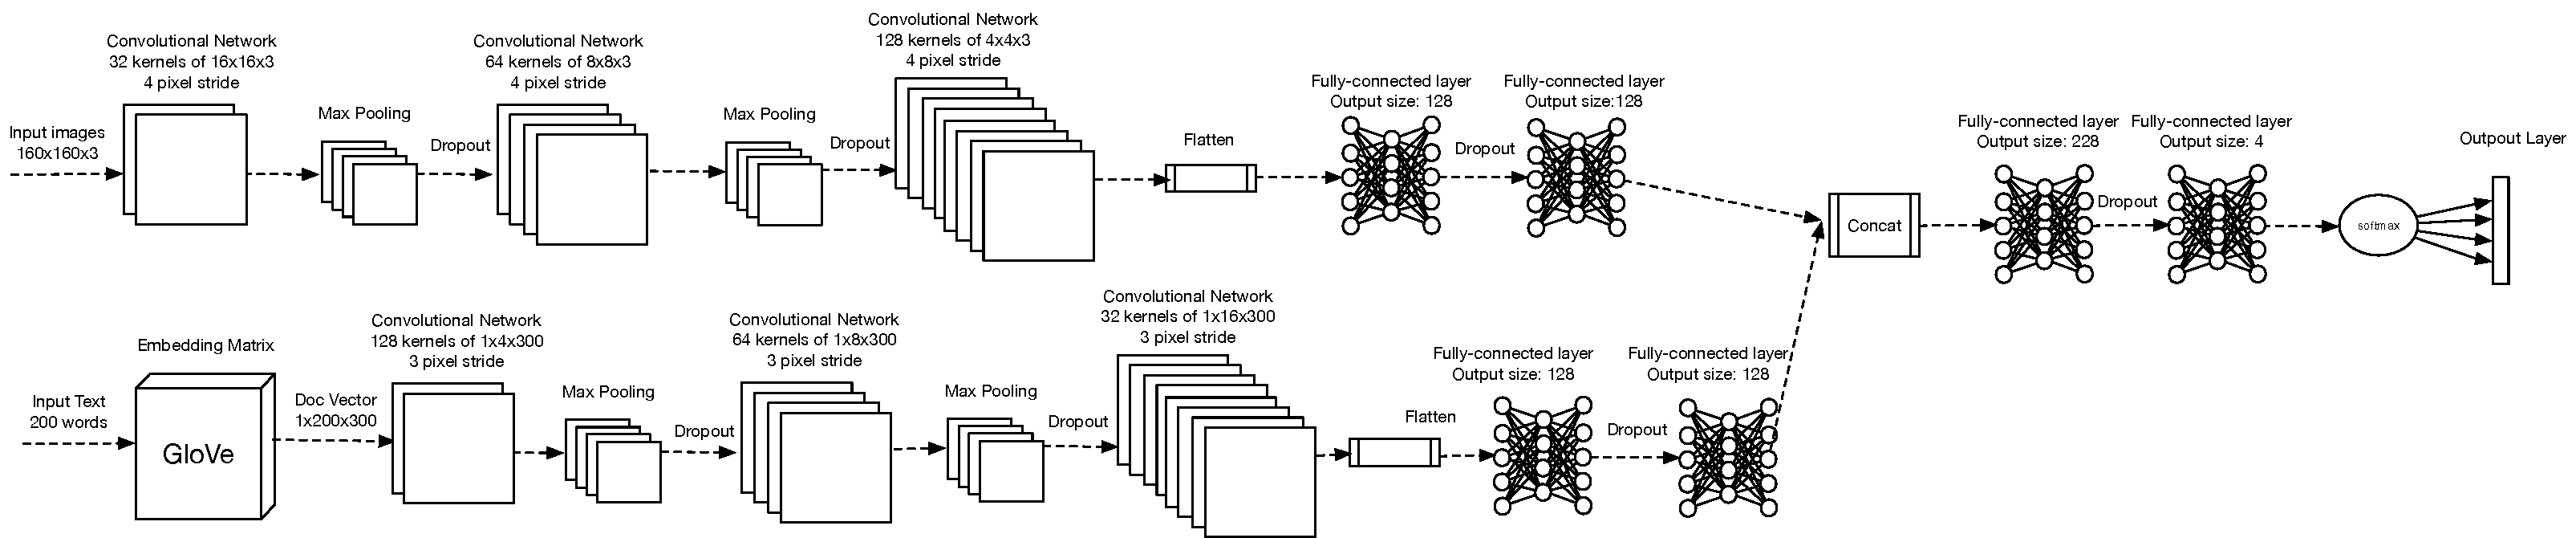
\includegraphics[totalheight=3cm]{Combined}
    \caption{Text classification neural network}
    \label{fig:CNN}
\end{figure}

\subsection{Proposed Neural Network}
  \label{ProposedNet}

Our network as depicted in Figure~\ref{fig:CNN} first receives the HTML document and the Image of the web page. It then feeds the input into the two separate CNNs. If either the HTML document is blank we feed a $1\times200\times300$ zero vector to the text classification CNN and the associating screenshot to the image classification CNN. There exists cases where we have the legitimate HTML document of the web page but the screenshot is a white picture, we proceed as before and feed each of the inputs to the appropriate CNN. Our model concatenates the output of the second fully-connected layer of both inputs and feeds
them as an input to another fully-connected layer we again apply a dropout of $0.5$ and go through one last fully-connected layer. A $4$-way softmax function is applied to the output of the last fully-connected layer to predict the class label.

\section{Datasets} 
\label{datasets}
We use an automated Selenium based web crawler written in Python for collecting screenshots and the HTML documents of Alexa\footnote{https://www.alexa.com/topsites} top $500$ web pages from a control host and 50 Tor~\cite{tor} exit relays located in 23 countries. Our control host does not connect to Tor exit relays and is located in an uncensored network in the US. Our crawls took place in November of 2017 and the dataset consists of $21246$ screenshots and their associated HTML documents. Glancing at the screenshots we can clearly see $4$ types of pages. (1) the Tor user can access the website like a non-Tor user which we see in Figure~\ref{fig:okpage}, we label these pages as \textit{ok}. (2) the Tor user reaches a server error page which we label with \textit{servererror} an example of these pages is shown in Figure~\ref{fig:servererror}. (3) the Tor user gets a connection failed or timeout page, we label these as \textit{connectionerror}. A sample connection error page is depicted in Figure~\ref{fig:connectionerror} and finally (4) the Tor user gets a block page or a page containing some form of CAPTCHA which we label as \textit{block} that can be seen in Figure~\ref{fig:blockpage}.
Our images have variable-resolutions, therefore we rescale our images to $160\times160$. We do not crop the center of each image, because many of the server error pages have content shown in the top part of the page. No pre-processing or data augmentation is done on our data and we only use the raw RGB values of the pixels as our image inputs. For the HTML documents, we take out the \textit{body} section of the page and parse over the first 200 words and provide this as our text inputs. This is because of the fact that the text content in an HTML document is available in the body section. We manually label our dataset by knowing that block pages usually have less length than a normal page~\cite{imc14_phillipa}.

\begin{figure}
    \centering
    \begin{subfigure}[b]{0.2\textwidth}
        \centering
        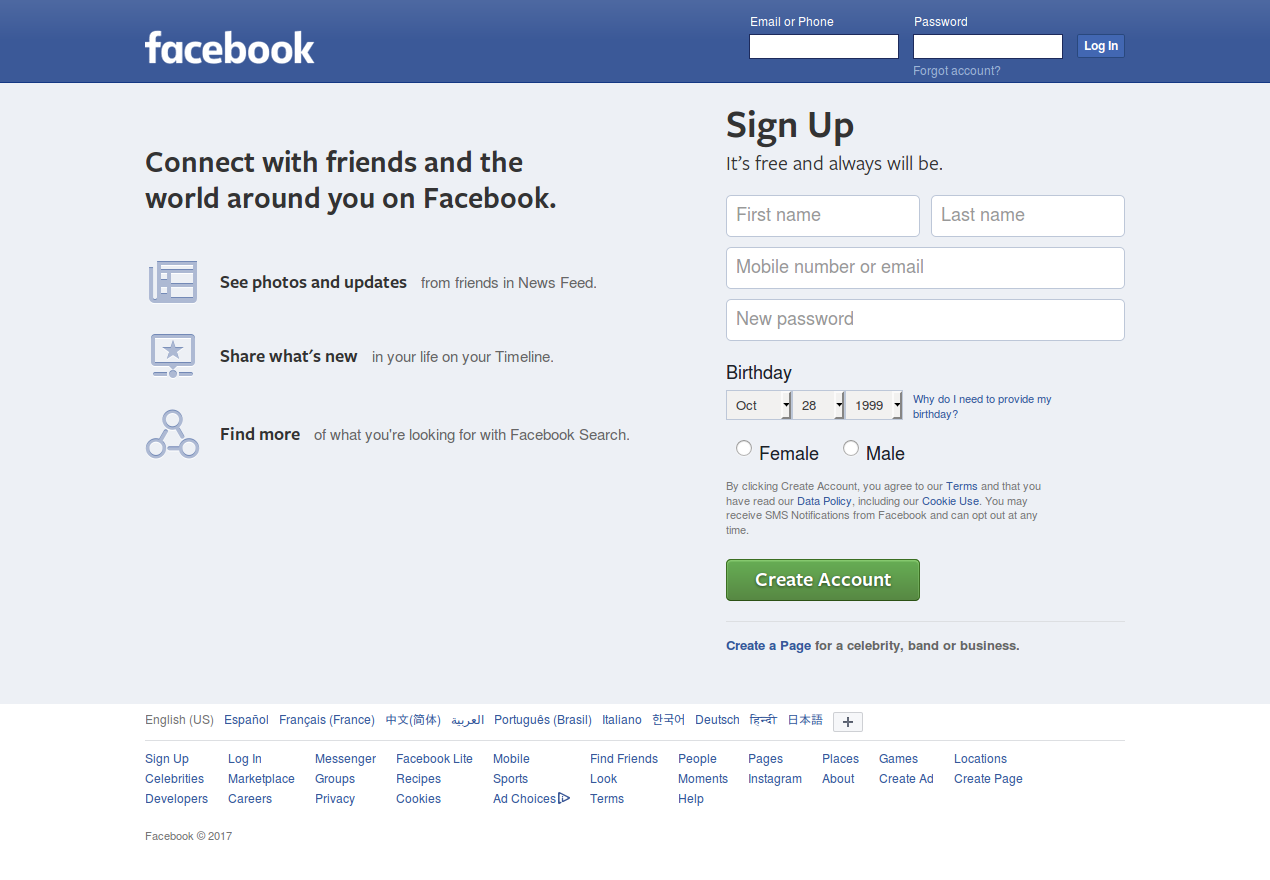
\includegraphics[width=\textwidth]{ok.png}
        \caption{Ok web page}
        \label{fig:okpage}
    \end{subfigure}
    \hfill
    \begin{subfigure}[b]{0.2\textwidth}
        \centering
        
\includegraphics[width=\textwidth]{block.png}
        \caption{Block page}
        \label{fig:blockpage}
    \end{subfigure}
    \hfill
        \hfill
    \begin{subfigure}[b]{0.2\textwidth}
        \centering
        
\includegraphics[width=\textwidth]{connectionerr.png}
        \caption{Connection error page}
        \label{fig:connectionerror}
    \end{subfigure}
    \hfill
    \begin{subfigure}[b]{0.2\textwidth}
        \centering
        
\includegraphics[width=\textwidth]{servererr.png}
        \caption{Server error page}
        \label{fig:servererror}
    \end{subfigure}
    \caption{Samples of our dataset}
    \label{fig:sample_dataset}
\end{figure}
\section{Experiments}
\label{experiments}
In order to evaluate the performance of our proposed model, we compare it with (1) CNN for image classification (2) CNN for text classification (3) prior work for block page detection (length difference) using a set of performance metrics. We conduct all the experiments on the previously mentioned dataset where we take 80\% of the data randomly as training and set aside the remaining 20\% for the test phase. Out of the 80\% for training, 25\% is also set for validation. Our hypothesis is that the our designed CNN should perform better than the CNNs for image and text classification. The reason being that there are cases where either the image or the text is missing for a data case and our proposed CNN would be more beneficial than a single CNN only focusing on text or image. Finally, previous techniques for block page detection were only heuristic based and had false positives, our method is designed to classify web pages into 4 distinct classes more accurately. In all experiments, the training batch size, validation batch size and test batch size are 607, 85 and 607 respectively.

\subsection{Performance Metrics}
We can not consider accuracy as the performance metric of our prediction, because our dataset is unbalanced. Meaning that the number of \textit{ok} pages is much more than the other classes. Hence, we select precision, recall, F1 score and macro-average F1 score as our performance metrics. The formulas are also shown in ~\ref{eqn:eqlabel}. These performance metrics have been used to evaluate block page detection in prior work as well ~\cite{imc14_phillipa}. In this work, $tp_c$(True Positives) is the number of correctly predicted cases of class $c$, $fp_c$(False Positives) is the number of cases that are incorrectly predicted as class $c$ and $fn_c$(False Negatives) is the number of cases belonging to class $c$ that the classifier failed to classify. The macro-average F1 score is the average F1 score over all classes, this is important to us because our classes do not have the same number of instances and the macro-averaged F1 gives equal weight to all classes.
 \begin{align}
\label{eqn:eqlabel}
\begin{split}
 precision_c = \dfrac{tp_c}{tp_c+fp_c} , \quad 
recall_c = \dfrac{tp_c}{tp_c+fn_c}, \quad 
\end{split}
\end{align}


 \begin{align}
\label{eqn:eqlabel2}
\begin{split}
F1_c = 2 \cdot \dfrac{precision_c \cdot recall_c}{precision_c + recall_c} \quad
F1_{macro-averaged} = \dfrac{\sum_{c=1}^{C} F1_c}{C}
\end{split}
\end{align}



\subsection{Hyper-parameters and Training}
We perform a grid search for hyper-parameter tuning. More specifically, we take the learning rate ($\alpha$) and the structure of the fully-connected layers in the networks as our hyper-parameters. For the learning rate, we consider $0.001$ and $0.0001$ values and for the fully-connected layers we consider: the case where we described our model architecture in ~\ref{ProposedNet} which we indicate with (1) for the rest of this paper and the case where we change the output size of the first fully-connected layer after the flatten process to $256$ then we add another fully-connected layer with the output size of $128$, finally we pass through another fully-connected layer with output size $4$, we specify this case with (2) for the rest of this paper. Therefore, for each experiment we will consider the effect of these hyper-parameters. We also apply a early stopping technique to our experiments. If the value of validation loss does not improve in $7$ subsequent epochs we do not continue and report the performance metric values when running our test data on the model's best weights.The results are shown in table~\ref{tab:hyperparam}
\section{Results}
After applying hyper-parameter tuning on our approach and the image and text classification CNNs we can compare their results on the same test set for evaluating the experiments mentioned in section~\ref{experiments}. For detecting \textit{ok} pages and \textit{block pages}, the image CNN works best with $\alpha=0.0001$ and the alternative fully-connected layer design(2), our proposed model performs best with  $\alpha=0.0001$ and the text CNN works is optimized with $\alpha=0.0001$ and the default design(1). The highest F1 score for each class is specified using a bold font in table~\ref{tab:hyperparam}.
\begin{figure*}
        \centering
        \begin{subfigure}[b]{0.48\textwidth}
            \centering
            \includegraphics[width=\textwidth]{okF1.png}
            \caption[]%
            {{\small Ok class}}    
            \label{fig:okF1}
        \end{subfigure}
        \hfill
        \begin{subfigure}[b]{0.48\textwidth}  
            \centering 
            \includegraphics[width=\textwidth]{blockF1.png}
            \caption[]%
            {{\small Block page class}}
            \label{fig:blockF1}
        \end{subfigure}
        \vskip\baselineskip
        \begin{subfigure}[b]{0.48\textwidth}   
            \centering 
            \includegraphics[width=\textwidth]{connectionF1.png}
            \caption[]%
            {{\small Connection error class}}    
            \label{fig:connectionF1}
        \end{subfigure}
        \quad
        \begin{subfigure}[b]{0.48\textwidth}   
            \centering 
            \includegraphics[width=\textwidth]{ServerF1.png}
            \caption[]%
            {{\small Server error class}}    
            \label{fig:serverF1}
        \end{subfigure}
        \caption[ F1 score vs number of epoch for each category ]
        {\small F1 score vs number of epoch for each category} 
        \label{fig:F1epoch}
        \vspace{-0.4cm}

    \end{figure*}
For evaluating our experiments, we train each of the models, namely the image CNN, text CNN and our proposed CNN with their optimized hyper-parameters and compare the F1 score of each of the 4 classes and the macro-averaged F1 score for all the classes. For the \textit{ok} and \textit{block page} classes, our proposed model gets a $0.998$ and $0.99$ F1 scores, which is higher than the text CNN and is the same as the image CNN but with fewer epochs. For the \textit{server error page} class, all models perform the same but our proposed model has the least number of epochs by $35$. Finally, for the \textit{connection error} pages, the Image CNN seems to outperform the other two. The macro-average F1 score for the Image CNN, text CNN and our proposed model are $0.985$, $0.9456$ and $0.981$ respectively. This shows that the Image CNN outperforms the two other models and our proposed model performs close to the image CNN and better than the text CNN. However, this might because of the fact that our data set does not have many missing images of web pages.
Figure~\ref{fig:F1epoch} plots the F1 score of each class vs the number of epochs each model had to train in order to obtain the results. Since we have more training data for the \textit{ok} class, we see that in Figure~\ref{fig:okF1} the starting F1 score is about $0.85$ which is relatively high. Whereas, for the other classes the F1 score starts from $0$.
In order to ensure that the training converges without overfitting, we have plotted the training and validation loss values of our 
   
\begin{table}
  \centering
  \resizebox{\columnwidth}{!}{%
  \begin{tabular}{|c|c|c|c|c|c|c|c|c|c|c|c|c|c|c|c|}
    \hline
    \multicolumn{1}{|>{{}}c|}{}&\multicolumn{3}{c|}{Ok page}&\multicolumn{3}{c|}{Block page}&\multicolumn{3}{c|}{Server error page}&\multicolumn{3}{c|}{Connection error page}&\multicolumn{1}{c|}{Epoch}\\
    \arrayrulecolor{}
    \arrayrulecolor{black}
    \cline{2-4}     \cline{5-7} \cline{8-10}\cline{11-13}

    \multicolumn{1}{|>{}c|}{Model}&Precision&Recall&F1&Precision&Recall&F1&Precision&Recall&F1&Precision&Recall&F1& \\
    \hline
    Image (1) $\alpha = 0.001$ &0.997&0.998&0.998&0.993&0.988&0.99&0.98&0.962&\bf{0.971}&0.981&0.981&0.981&92\\
    \hline
         Image (2)  $\alpha =0.001$&0.996&0.998&0.997&0.986&0.979&0.982&0.971&0.962&0.966&0.993&0.981&\bf{0.987}&85\\
    \hline
     Image (1)   $\alpha =0.0001$&0.99&0.99&0.99&0.988&0.97&0.979&0.953&0.962&0.957&0.993&0.981&0.987&91\\
    \hline
    Image (2)    $\alpha =0.0001$&0.998&0.998&\bf{0.998}&0.993&0.988&\bf{0.99}&0.935&0.962&0.948&0.987&0.981&0.984&115\\
    \hline
        HTML (1) $\alpha =0.001$ &0.981&0.999&0.99&0.995&0.935&0.964&0.98&0.962&0.971&0.991&0.759&0.86&59\\
    \hline
         HTML (2)  $\alpha =0.001$&0.982&1.0&0.99&0.997&0.938&0.96&0.98&0.96&\bf{0.971}&0.99&0.759&\bf{0.86}&95\\
    \hline
     HTML (1)   $\alpha =0.0001$&0.982&1.0&\bf{0.99}&1.0&0.938&\bf{0.968}&0.971&0.962&0.966&0.991&0.759&0.86&125\\
    \hline
    HTML (2)    $\alpha =0.0001$&0.981&0.999&0.99&0.997&0.935&0.965&0.971&0.962&0.966&0.991&0.759&0.86&105\\
    \hline
            Our model (1) $\alpha =0.001$ &0.995&0.999&0.997&0.995&0.983&0.99&0.98&0.962&\bf{0.971}&0.98&0.95&0.965&57\\
    \hline
            Our model (2)  $\alpha =0.001$&0.997&0.998&0.998&0.995&0.965&0.0.98&0.962&0.971&0.967&0.939&0.981&0.959&98\\
    \hline
            Our model (1)   $\alpha =0.0001$&0.998&0.999&\bf{0.998}&0.997&0.983&\bf{0.99}&0.971&0.952&0.962&0.968&0.981&\bf{0.974}&92\\
    \hline
            Our model (2)    $\alpha =0.0001$&0.997&0.999&0.998&0.997&0.933&0.964&0.971&0.962&0.966&0.829&0.987&0.90&67\\
    \hline
             Length difference (2)    $\alpha =0.0001$&0.93&0.71&0.80&0.31&1.0&0.47&0&0&0&0&0&0&0\\
    \hline
  \end{tabular}
  }
  \caption{Performance metrics in various scenarios}
  \label{tab:hyperparam}
\end{table}


\begin{figure}
    \centering
    \begin{subfigure}[b]{0.3\textwidth}
        \centering
        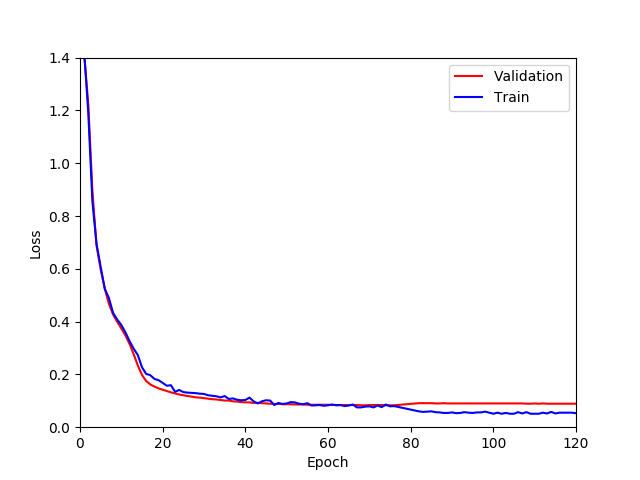
\includegraphics[width=\textwidth]{html_val_train.png}
        \caption{Text CNN}
        \label{fig:blockpage}
    \end{subfigure}
    \hfill
        \hfill
    \begin{subfigure}[b]{0.3\textwidth}
        \centering
        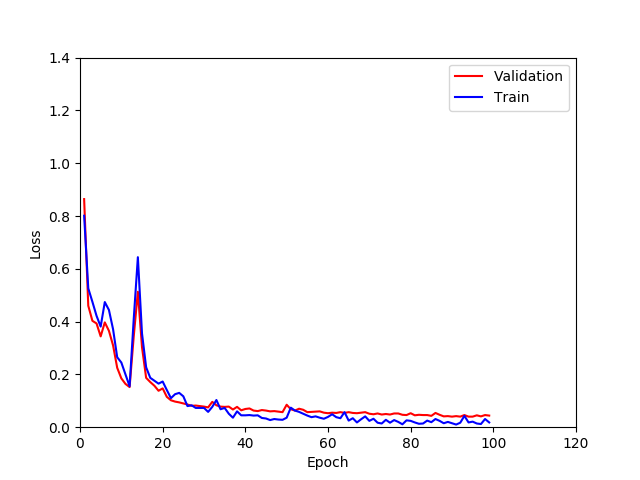
\includegraphics[width=\textwidth]{png_val_train.png}
        \caption{Image CNN}
        \label{fig:connectionerror}
    \end{subfigure}
   \hfill
    \begin{subfigure}[b]{0.3\textwidth}
        \centering
        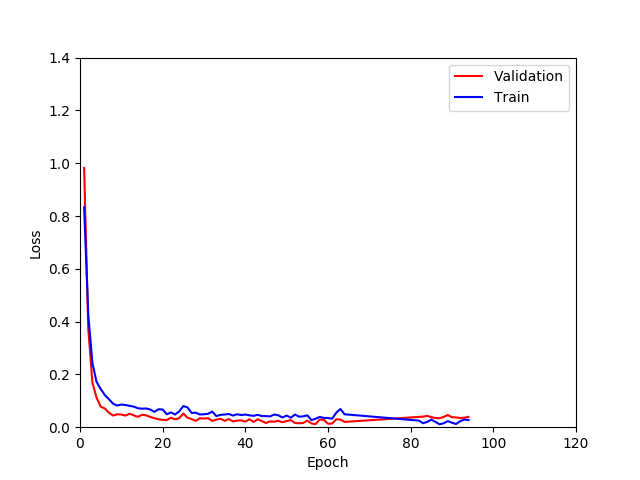
\includegraphics[width=\textwidth]{model_val_train.png}
        \caption{Proposed Model}
        \label{fig:servererror}
    \end{subfigure}
    \caption{Training and validation loss curves for the best settings of our $3$ experiments}
    \label{fig:sample_dataset}
\end{figure}


\section{Discussion and Conclusions}
\label{sec:discussion}
In this work, we design and implement a novel deep convolutional neural network which works with text and images simultaneously and apply it to the task of block page detection. We collect a data set of web page crawls consisting of $21246$ screenshots and HTML documents of the Alexa top 500 web pages from 50 Tor exit relays. We study and compare the performance of our proposed model on our data set, with an image convolutional neural network that works only with images, a textual convolutional neural network which only works with text and previous work on block page detection using heuristics. Our hypothesis is that our designed model will work better in cases when there are missing data in either the text or the screenshots. We use the F1 score as a performance metric to evaluate the models. Our results show that our the previous techniques on block page detection no longer work and our proposed model performs extremely better. and observe that our proposed model performs slightly better than the image CNN in fewer epochs.


\subsection{Future work}
Our proposed model can be extended by using stacked autoencoders with unlabeled data in order to learn high-level features ~\cite{icml_unsupervised}. Furthermore, by using data augmentation we can enlarge the data set and avoid overfitting by transforming the images and using a thesaurus to replace words with their synonyms ~\cite{icml_unsupervised}~\cite{nips_text}. We also plan to evaluate the model on larger data sets with more missing data.

%
%
%
%\subsubsection*{References}
%
%References follow the acknowledgments. Use unnumbered third level heading for
%the references. Any choice of citation style is acceptable as long as you are
%consistent. It is permissible to reduce the font size to `small' (9-point) 
%when listing the references. {\bf Remember that this year you can use
%a ninth page as long as it contains \emph{only} cited references.}
%
%\small{
%[1] Alexander, J.A. \& Mozer, M.C. (1995) Template-based algorithms
%for connectionist rule extraction. In G. Tesauro, D. S. Touretzky
%and T.K. Leen (eds.), {\it Advances in Neural Information Processing
%Systems 7}, pp. 609-616. Cambridge, MA: MIT Press.
%
%[2] Bower, J.M. \& Beeman, D. (1995) {\it The Book of GENESIS: Exploring
%Realistic Neural Models with the GEneral NEural SImulation System.}
%New York: TELOS/Springer-Verlag.
%
%[3] Hasselmo, M.E., Schnell, E. \& Barkai, E. (1995) Dynamics of learning
%and recall at excitatory recurrent synapses and cholinergic modulation
%in rat hippocampal region CA3. {\it Journal of Neuroscience}
%{\bf 15}(7):5249-5262.
%}
\printbibliography
\end{document}